\documentclass[tikz]{standalone}
\usepackage{amsmath,amssymb}
\usetikzlibrary{arrows,automata,petri,trees}

\tikzstyle{b} = [circle, white, font=\bf\tt, draw=black, fill=black, align=center, inner sep=0pt, text width=1.5em, text centered]
\tikzstyle{r} = [circle, white, font=\bf\tt, draw=red,   fill=red,   align=center, inner sep=0pt, text width=1.5em, text centered]

\tikzstyle{n} = [rectangle, white, draw=black, align=center, inner sep=0pt, minimum width=0.5em, minimum height=0.5em]

\tikzstyle{o} = [circle, orange, draw=orange, align=center, inner sep=0.85em, very thick]
\tikzstyle{t} = [circle, teal,   draw=teal,   align=center, inner sep=0.85em, very thick]

\tikzstyle{h} = [blue, very thick]
\tikzstyle{n} = [black, thin]

\begin{document}
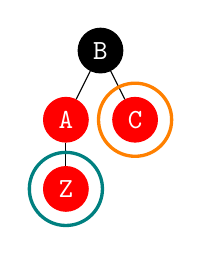
\begin{tikzpicture}[level distance=25pt,sibling distance=25pt]
	\node [b] {B}
	child { node [r] {A}
			child { node [r] {Z} node [t] {~} }
		}
	child { node [r] {C} node [o] {~} };
\end{tikzpicture}
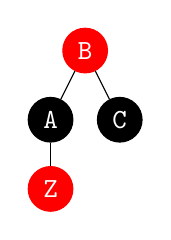
\begin{tikzpicture}[level distance=25pt,sibling distance=25pt]
	\node [r] {B}
	child { node [b] {A}
			child { node [r] {Z} }
		}
	child { node [b] {C} };
\end{tikzpicture}
%% ========================================================
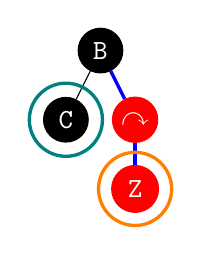
\begin{tikzpicture}[level distance=25pt,sibling distance=25pt]
	\node [b] {B}
	child { node [b] {C} node [t] {~} }
	child [h] { node [r] {\(\curvearrowright\)}
			child [h]{ node [r] {Z} node [o] {~} }
		};
\end{tikzpicture}
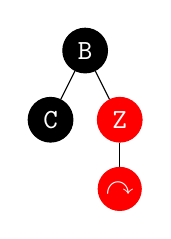
\begin{tikzpicture}[level distance=25pt,sibling distance=25pt]
	\node [b] {B}
	child { node [b] {C} }
	child { node [r] {Z}
			child { node [r] {\(\curvearrowright\)} }
		};
\end{tikzpicture}
%% ========================================================
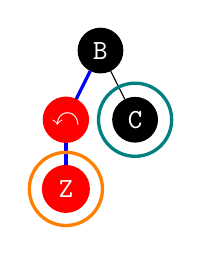
\begin{tikzpicture}[level distance=25pt,sibling distance=25pt]
	\node [b] {B}
	child [h] { node [r] {\(\curvearrowleft\)}
			child [h] { node [r] {Z} node [o] {~} }
		}
	child { node [b] {C} node [t] {~} };
\end{tikzpicture}
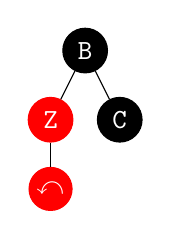
\begin{tikzpicture}[level distance=25pt,sibling distance=25pt]
	\node [b] {B}
	child { node [r] {Z}
			child { node [r] {\(\curvearrowleft\)} }
		}
	child { node [b] {C} };
\end{tikzpicture}
%% ========================================================
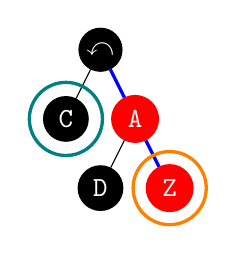
\begin{tikzpicture}[level distance=25pt,sibling distance=25pt]
	\node [b] {\(\curvearrowleft\)}
	child { node [b] {C} node [t] {~} }
	child [h] { node [r] {A}
			child [n] { node [b] {D} }
			child [h] { node [r] {Z} node [o] {~} }
		};
\end{tikzpicture}
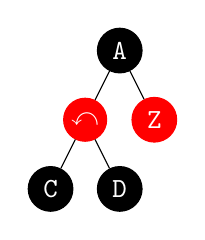
\begin{tikzpicture}[level distance=25pt,sibling distance=25pt]
	\node [b] {A}
	child { node [r] {\(\curvearrowleft\)}
			child { node [b] {C} }
			child { node [b] {D} }
		}
	child { node [r] {Z} };
\end{tikzpicture}
%% ========================================================
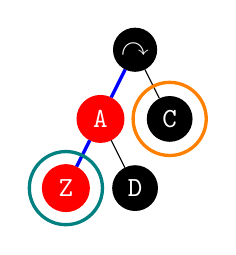
\begin{tikzpicture}[level distance=25pt,sibling distance=25pt]
	\node [b] {\(\curvearrowright\)}
	child [h] { node [r] {A}
			child [h] { node [r] {Z} node [t] {~} }
			child [n] { node [b] {D} }
		}
	child { node [b] {C} node [o] {~} };
\end{tikzpicture}
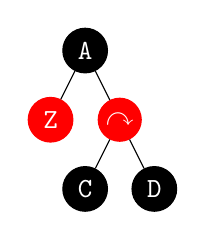
\begin{tikzpicture}[level distance=25pt,sibling distance=25pt]
	\node [b] {A}
	child { node [r] {Z} }
	child  { node [r] {\(\curvearrowright\)}
			child { node [b] {C} }
			child { node [b] {D} }
		};
\end{tikzpicture}
\end{document}